\begin{figure}[t]
    \centering
    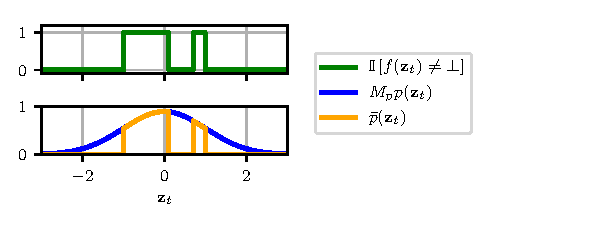
\includegraphics[width=0.45\textwidth]{figures/explanatory-plot.pdf}
    \vspace{-0.3cm}
    \caption{Graphical representation of how a brittle deterministic simulator acts as a rejection sampler, targeting $\overline{p}(\mathbf{z}_t | \mathbf{x}_{t-1})$.
    We set $\mathbf{x}_t = 0$ for clarity.
    The simulator, $f(\mathbf{z}_t)$, returns $\bot$ for unknown input regions, shown in green.
    The proposal over $\mathbf{z}_t$ is shown in blue.
    The target distribution, $\overline{p}(\mathbf{z}_t)$, shown in orange, is implicitly defined as $\overline{p}(\mathbf{z}_t) = \frac{1}{M_p} p(\mathbf{z}_t) \mathbb{I}\left[ f(\mathbf{z}_t) \neq \bot \right]$, where $M_p$ is the normalizing constant from $\overline{p}$, equal to the acceptance rate.
    Accordingly, the proposal distribution, scaled by $M_p$, is \emph{exactly} equal to $\overline{p}(\mathbf{z}_t)$ in the accepted region.
    Algorithm \ref{alg:rs} therefore implicitly constructs a rejection sampler, where the acceptance criterion reduces to $\mathbb{I}\left[ f(\mathbf{z}_t) \neq \bot \right]$, without needing to specify any additional scaling constants.
    }
    \label{fig:rs}
\end{figure}